\documentclass[11pt,a4paper]{article}

% Packages
\usepackage[utf8]{inputenc}
\usepackage[T1]{fontenc}
\usepackage{geometry}
\usepackage{amsmath,amssymb}
\usepackage{graphicx}
\usepackage{xcolor}
\usepackage{enumitem}
\usepackage{tcolorbox}
\usepackage{tikz}
\usepackage[hidelinks]{hyperref}
\usepackage{fancyhdr}
\usepackage{titlesec}
\usepackage{booktabs}
\usepackage{array}
\usepackage{listings}
\usepackage{multicol}
\usepackage{mdframed}

% Page geometry
\geometry{margin=0.9in}
\setlength{\headheight}{14pt}

% Colors
\definecolor{pytorchcolor}{RGB}{238,76,44}
\definecolor{conceptbg}{RGB}{240,248,255}
\definecolor{codebg}{RGB}{248,248,248}
\definecolor{importantbg}{RGB}{255,250,230}
\definecolor{tipbg}{RGB}{240,255,240}
\definecolor{warningbg}{RGB}{255,245,245}
\definecolor{codegreen}{RGB}{0,128,0}
\definecolor{codegray}{RGB}{128,128,128}
\definecolor{formulabg}{RGB}{245,245,255}

% Code listing style
\lstset{
    language=Python,
    basicstyle=\ttfamily\small,
    keywordstyle=\color{pytorchcolor}\bfseries,
    commentstyle=\color{codegray}\itshape,
    stringstyle=\color{codegreen},
    breaklines=true,
    frame=single,
    backgroundcolor=\color{codebg},
    showstringspaces=false,
    tabsize=4,
    morekeywords={torch,nn,optim,self,True,False,None,optuna,lightning,pl}
}

% Custom boxes
\tcbuselibrary{skins,breakable}

\newtcolorbox{conceptbox}[1][]{
    colback=conceptbg,
    colframe=blue!60!black,
    fonttitle=\bfseries,
    title=#1,
    breakable
}

\newtcolorbox{importantbox}[1][Key Concept]{
    colback=importantbg,
    colframe=orange!70!black,
    fonttitle=\bfseries,
    title=#1,
    breakable
}

\newtcolorbox{tipbox}[1][Tip]{
    colback=tipbg,
    colframe=green!60!black,
    fonttitle=\bfseries,
    title=#1,
    breakable
}

\newtcolorbox{warningbox}[1][Warning]{
    colback=warningbg,
    colframe=red!60!black,
    fonttitle=\bfseries,
    title=#1,
    breakable
}

\newtcolorbox{formulabox}[1][Formula]{
    colback=formulabg,
    colframe=purple!60!black,
    fonttitle=\bfseries,
    title=#1,
    breakable
}

% Header/Footer
\pagestyle{fancy}
\fancyhf{}
\fancyhead[L]{\textcolor{pytorchcolor}{\textbf{Course 2: Intermediate PyTorch}}}
\fancyhead[R]{PyTorch Specialization}
\fancyfoot[C]{\thepage}

% Title formatting
\titleformat{\section}{\Large\bfseries\color{pytorchcolor}}{\thesection}{1em}{}
\titleformat{\subsection}{\large\bfseries\color{blue!70!black}}{\thesubsection}{1em}{}
\titleformat{\subsubsection}{\normalsize\bfseries\color{black!70}}{\thesubsubsection}{1em}{}

\begin{document}

% Title Page
\begin{titlepage}
    \centering
    \vspace*{1.5cm}
    
    {\Huge\bfseries\color{pytorchcolor} Course 2\\[0.3cm]}
    {\LARGE Intermediate PyTorch\\[1.5cm]}
    
    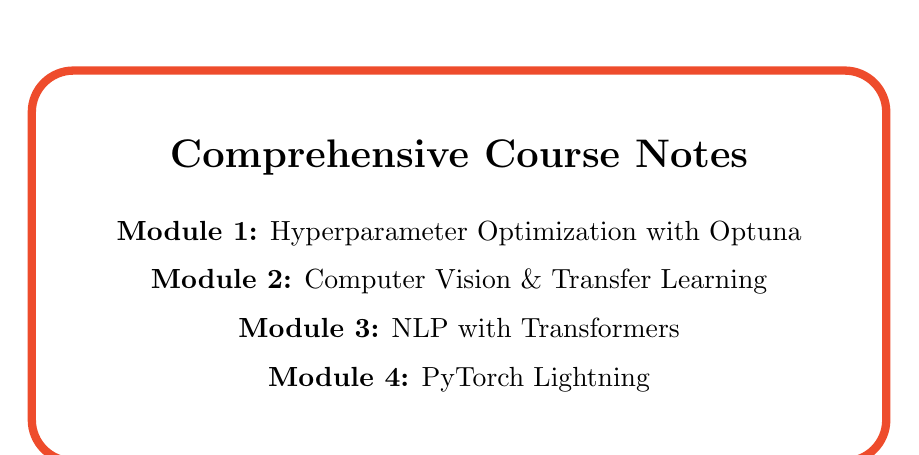
\begin{tikzpicture}
        \node[draw=pytorchcolor, line width=3pt, rounded corners=15pt, inner sep=25pt, fill=white] {
            \begin{minipage}{0.75\textwidth}
                \centering
                \Large\textbf{Comprehensive Course Notes}\\[0.5cm]
                \normalsize
                \textbf{Module 1:} Hyperparameter Optimization with Optuna\\[0.2cm]
                \textbf{Module 2:} Computer Vision \& Transfer Learning\\[0.2cm]
                \textbf{Module 3:} NLP with Transformers\\[0.2cm]
                \textbf{Module 4:} PyTorch Lightning
            \end{minipage}
        };
    \end{tikzpicture}
    
    \vfill
    
    \begin{tikzpicture}
        \draw[pytorchcolor, line width=2pt] (0,0) -- (12,0);
    \end{tikzpicture}
    
    \vspace{1cm}
    {\large PyTorch Deep Learning Specialization}\\[0.5cm]
    {\large\today}
\end{titlepage}

% Table of Contents
\tableofcontents
\newpage

%==============================================================================
% MODULE 1: HYPERPARAMETER OPTIMIZATION
%==============================================================================
\section{Module 1: Hyperparameter Optimization with Optuna}

\subsection{Introduction to AutoML}

\begin{conceptbox}[What is AutoML?]
AutoML (Automated Machine Learning) automates the machine learning pipeline:
\begin{itemize}
    \item Feature engineering
    \item Model selection
    \item \textbf{Hyperparameter optimization} $\leftarrow$ Focus of this module
    \item Architecture search
\end{itemize}
\end{conceptbox}

\subsection{Optuna Framework}

\begin{importantbox}[Optuna Key Concepts]
\begin{itemize}
    \item \textbf{Study:} A complete optimization session
    \item \textbf{Trial:} A single training run with specific hyperparameters
    \item \textbf{Objective Function:} Returns the metric to optimize
    \item \textbf{Sampler:} Strategy for selecting hyperparameters (TPE, Random, etc.)
    \item \textbf{Pruner:} Early stops unpromising trials
\end{itemize}
\end{importantbox}

\begin{lstlisting}[caption=Basic Optuna Setup]
import optuna

def objective(trial):
    # Suggest hyperparameters
    lr = trial.suggest_float("lr", 1e-5, 1e-1, log=True)
    n_layers = trial.suggest_int("n_layers", 1, 5)
    dropout = trial.suggest_float("dropout", 0.1, 0.5)
    
    # Build model with suggested params
    model = build_model(n_layers, dropout)
    
    # Train and evaluate
    accuracy = train_and_evaluate(model, lr)
    
    return accuracy  # Optuna will maximize/minimize this

# Create and run study
study = optuna.create_study(direction="maximize")
study.optimize(objective, n_trials=100)

# Best hyperparameters
print(study.best_params)
print(study.best_value)
\end{lstlisting}

\subsection{Suggest Methods}

\begin{center}
\begin{tabular}{lp{7cm}}
\toprule
\textbf{Method} & \textbf{Usage} \\
\midrule
\texttt{suggest\_int(name, low, high)} & Integer values \\
\texttt{suggest\_float(name, low, high)} & Float values \\
\texttt{suggest\_float(..., log=True)} & Log-scale sampling (for learning rates) \\
\texttt{suggest\_categorical(name, choices)} & Choose from list of options \\
\bottomrule
\end{tabular}
\end{center}

\begin{lstlisting}[caption=Hyperparameter Suggestions]
def objective(trial):
    # Learning rate (log scale)
    lr = trial.suggest_float("lr", 1e-5, 1e-1, log=True)
    
    # Architecture choices
    n_filters = trial.suggest_int("n_filters", 16, 128)
    n_layers = trial.suggest_int("n_layers", 2, 6)
    
    # Regularization
    dropout = trial.suggest_float("dropout", 0.0, 0.5)
    
    # Categorical choice
    optimizer_name = trial.suggest_categorical(
        "optimizer", ["Adam", "SGD", "RMSprop"]
    )
    
    # Build and train model...
\end{lstlisting}

\subsection{FlexibleCNN Architecture}

\begin{lstlisting}[caption=Flexible CNN for Hyperparameter Search]
class FlexibleCNN(nn.Module):
    def __init__(self, n_layers, n_filters, dropout_rate, num_classes):
        super().__init__()
        
        layers = []
        in_channels = 3
        
        for i in range(n_layers):
            out_channels = n_filters * (2 ** i)  # Double channels
            layers.extend([
                nn.Conv2d(in_channels, out_channels, 3, padding=1),
                nn.BatchNorm2d(out_channels),
                nn.ReLU(),
                nn.MaxPool2d(2, 2)
            ])
            in_channels = out_channels
        
        self.features = nn.Sequential(*layers)
        self.flatten = nn.Flatten()
        
        # Calculate flattened size
        with torch.no_grad():
            dummy = torch.zeros(1, 3, 32, 32)
            flat_size = self.features(dummy).view(1, -1).size(1)
        
        self.classifier = nn.Sequential(
            nn.Linear(flat_size, 256),
            nn.ReLU(),
            nn.Dropout(dropout_rate),
            nn.Linear(256, num_classes)
        )
    
    def forward(self, x):
        x = self.features(x)
        x = self.flatten(x)
        return self.classifier(x)
\end{lstlisting}

\subsection{Pruning Unpromising Trials}

\begin{tipbox}[Median Pruner]
Stops trials that perform worse than the median of completed trials at the same step:
\begin{lstlisting}
study = optuna.create_study(
    direction="maximize",
    pruner=optuna.pruners.MedianPruner(
        n_startup_trials=5,
        n_warmup_steps=5
    )
)
\end{lstlisting}
\end{tipbox}

\begin{lstlisting}[caption=Reporting for Pruning]
def objective(trial):
    model = build_model(trial)
    
    for epoch in range(num_epochs):
        train_loss = train_one_epoch(model)
        val_acc = evaluate(model)
        
        # Report intermediate value for pruning
        trial.report(val_acc, epoch)
        
        # Check if trial should be pruned
        if trial.should_prune():
            raise optuna.TrialPruned()
    
    return val_acc
\end{lstlisting}

\subsection{Study Persistence}

\begin{lstlisting}[caption=Saving and Loading Studies]
# Save to SQLite database
study = optuna.create_study(
    study_name="cnn_optimization",
    storage="sqlite:///optuna_study.db",
    load_if_exists=True  # Resume existing study
)

# Continue optimization
study.optimize(objective, n_trials=50)

# Analyze results
print(f"Best trial: {study.best_trial.number}")
print(f"Best params: {study.best_params}")
print(f"Best value: {study.best_value}")

# Get all trials
df = study.trials_dataframe()
\end{lstlisting}

\subsection{Visualization}

\begin{lstlisting}[caption=Optuna Visualization]
import optuna.visualization as vis

# Parameter importance
vis.plot_param_importances(study)

# Optimization history
vis.plot_optimization_history(study)

# Parameter relationships
vis.plot_parallel_coordinate(study)

# Hyperparameter slice
vis.plot_slice(study)
\end{lstlisting}

\newpage
%==============================================================================
% MODULE 2: COMPUTER VISION & TRANSFER LEARNING
%==============================================================================
\section{Module 2: Computer Vision \& Transfer Learning}

\subsection{What is Transfer Learning?}

\begin{conceptbox}[Transfer Learning]
Using a model pretrained on a large dataset (e.g., ImageNet) and adapting it to a new task:
\begin{itemize}
    \item Leverages learned features (edges, textures, objects)
    \item Requires less data for the new task
    \item Faster training convergence
    \item Often achieves better results than training from scratch
\end{itemize}
\end{conceptbox}

\subsection{TorchVision Models}

\begin{lstlisting}[caption=Loading Pretrained Models]
import torchvision.models as models

# Load pretrained model
model = models.mobilenet_v3_small(weights='IMAGENET1K_V1')

# Alternative models
resnet18 = models.resnet18(weights='IMAGENET1K_V1')
efficientnet = models.efficientnet_b0(weights='IMAGENET1K_V1')
vgg16 = models.vgg16(weights='IMAGENET1K_V1')
\end{lstlisting}

\begin{importantbox}[Model Selection Considerations]
\begin{itemize}
    \item \textbf{MobileNetV3:} Lightweight, fast, mobile-friendly
    \item \textbf{ResNet:} Reliable, well-understood, various depths
    \item \textbf{EfficientNet:} Best accuracy/efficiency tradeoff
    \item \textbf{VGG:} Simple architecture, good for visualization
\end{itemize}
\end{importantbox}

\subsection{Modifying for Custom Tasks}

\begin{lstlisting}[caption=Replacing the Classifier]
# MobileNetV3
model = models.mobilenet_v3_small(weights='IMAGENET1K_V1')
num_classes = 10

# Get number of input features to classifier
in_features = model.classifier[0].in_features

# Replace classifier
model.classifier = nn.Sequential(
    nn.Linear(in_features, 256),
    nn.Hardswish(),
    nn.Dropout(p=0.2),
    nn.Linear(256, num_classes)
)

# ResNet (replaces fc layer)
resnet = models.resnet18(weights='IMAGENET1K_V1')
resnet.fc = nn.Linear(resnet.fc.in_features, num_classes)
\end{lstlisting}

\subsection{Freezing Pretrained Weights}

\begin{lstlisting}[caption=Feature Extraction vs Fine-Tuning]
# Option 1: Feature Extraction (freeze all)
for param in model.parameters():
    param.requires_grad = False

# Unfreeze classifier only
for param in model.classifier.parameters():
    param.requires_grad = True

# Option 2: Gradual Unfreezing (fine-tune later layers)
# Freeze early layers
for name, param in model.named_parameters():
    if 'features.0' in name or 'features.1' in name:
        param.requires_grad = False
\end{lstlisting}

\begin{tipbox}[Freezing Strategy]
\begin{enumerate}
    \item Start with frozen backbone, train classifier only
    \item Gradually unfreeze later layers
    \item Use lower learning rate for pretrained weights
\end{enumerate}
\end{tipbox}

\subsection{ImageFolder Dataset}

\begin{lstlisting}[caption=Using ImageFolder]
from torchvision.datasets import ImageFolder

# Directory structure:
# data/
#   train/
#     class_a/
#     class_b/
#   val/
#     class_a/
#     class_b/

train_dataset = ImageFolder(
    root='data/train',
    transform=train_transform
)

val_dataset = ImageFolder(
    root='data/val',
    transform=val_transform
)

# Class names
print(train_dataset.classes)  # ['class_a', 'class_b']
print(train_dataset.class_to_idx)  # {'class_a': 0, 'class_b': 1}
\end{lstlisting}

\subsection{ImageNet Preprocessing}

\begin{lstlisting}[caption=Standard Preprocessing for Pretrained Models]
# ImageNet statistics
IMAGENET_MEAN = [0.485, 0.456, 0.406]
IMAGENET_STD = [0.229, 0.224, 0.225]

train_transform = transforms.Compose([
    transforms.Resize(256),
    transforms.RandomResizedCrop(224),
    transforms.RandomHorizontalFlip(),
    transforms.ToTensor(),
    transforms.Normalize(IMAGENET_MEAN, IMAGENET_STD)
])

val_transform = transforms.Compose([
    transforms.Resize(256),
    transforms.CenterCrop(224),
    transforms.ToTensor(),
    transforms.Normalize(IMAGENET_MEAN, IMAGENET_STD)
])
\end{lstlisting}

\subsection{Learning Rate Scheduling}

\begin{lstlisting}[caption=Learning Rate Schedulers]
from torch.optim.lr_scheduler import StepLR, ReduceLROnPlateau

# Step decay
scheduler = StepLR(optimizer, step_size=10, gamma=0.1)
# Reduce LR by 0.1 every 10 epochs

# Adaptive (reduce on plateau)
scheduler = ReduceLROnPlateau(
    optimizer, 
    mode='min',       # Minimize metric
    factor=0.1,       # Multiply LR by this
    patience=5,       # Wait this many epochs
    verbose=True
)

# In training loop
for epoch in range(num_epochs):
    train_loss = train_epoch(...)
    val_loss = validate(...)
    
    # For StepLR
    scheduler.step()
    
    # For ReduceLROnPlateau
    scheduler.step(val_loss)
\end{lstlisting}

\subsection{Differential Learning Rates}

\begin{lstlisting}[caption=Different LR for Different Layers]
# Lower LR for pretrained features, higher for new classifier
optimizer = optim.Adam([
    {'params': model.features.parameters(), 'lr': 1e-5},
    {'params': model.classifier.parameters(), 'lr': 1e-3}
])
\end{lstlisting}

\newpage
%==============================================================================
% MODULE 3: NLP WITH TRANSFORMERS
%==============================================================================
\section{Module 3: NLP with Transformers}

\subsection{Text Classification Pipeline}

\begin{conceptbox}[NLP Pipeline Steps]
\begin{enumerate}
    \item \textbf{Tokenization:} Convert text to tokens (words/subwords)
    \item \textbf{Encoding:} Convert tokens to numerical IDs
    \item \textbf{Embedding:} Map IDs to dense vectors
    \item \textbf{Processing:} Apply transformer/RNN layers
    \item \textbf{Classification:} Final prediction layer
\end{enumerate}
\end{conceptbox}

\subsection{Tokenization}

\begin{lstlisting}[caption=Basic Tokenization]
from transformers import AutoTokenizer

tokenizer = AutoTokenizer.from_pretrained('distilbert-base-uncased')

# Tokenize text
text = "I love PyTorch!"
tokens = tokenizer(
    text,
    padding='max_length',
    truncation=True,
    max_length=128,
    return_tensors='pt'
)

print(tokens['input_ids'].shape)      # [1, 128]
print(tokens['attention_mask'].shape) # [1, 128]
\end{lstlisting}

\begin{importantbox}[Tokenizer Output]
\begin{itemize}
    \item \textbf{input\_ids:} Token indices for the vocabulary
    \item \textbf{attention\_mask:} 1 for real tokens, 0 for padding
    \item \textbf{Special tokens:} [CLS] at start, [SEP] at end
\end{itemize}
\end{importantbox}

\subsection{DistilBERT for Classification}

\begin{lstlisting}[caption=Loading DistilBERT]
from transformers import DistilBertModel, DistilBertConfig

# Load pretrained DistilBERT
bert = DistilBertModel.from_pretrained('distilbert-base-uncased')

# Get hidden size
hidden_size = bert.config.hidden_size  # 768
\end{lstlisting}

\subsection{Custom Text Classifier}

\begin{lstlisting}[caption=Text Classification Model]
class TextClassifier(nn.Module):
    def __init__(self, num_classes, dropout=0.3):
        super().__init__()
        
        self.bert = DistilBertModel.from_pretrained(
            'distilbert-base-uncased'
        )
        self.dropout = nn.Dropout(dropout)
        self.classifier = nn.Linear(
            self.bert.config.hidden_size,  # 768
            num_classes
        )
    
    def forward(self, input_ids, attention_mask):
        # Get BERT output
        outputs = self.bert(
            input_ids=input_ids,
            attention_mask=attention_mask
        )
        
        # Use [CLS] token representation
        cls_output = outputs.last_hidden_state[:, 0, :]
        
        # Classify
        x = self.dropout(cls_output)
        logits = self.classifier(x)
        return logits
\end{lstlisting}

\subsection{Custom Dataset for Text}

\begin{lstlisting}[caption=Text Dataset Class]
class TextDataset(Dataset):
    def __init__(self, texts, labels, tokenizer, max_length=128):
        self.texts = texts
        self.labels = labels
        self.tokenizer = tokenizer
        self.max_length = max_length
    
    def __len__(self):
        return len(self.texts)
    
    def __getitem__(self, idx):
        encoding = self.tokenizer(
            self.texts[idx],
            padding='max_length',
            truncation=True,
            max_length=self.max_length,
            return_tensors='pt'
        )
        
        return {
            'input_ids': encoding['input_ids'].squeeze(0),
            'attention_mask': encoding['attention_mask'].squeeze(0),
            'label': torch.tensor(self.labels[idx], dtype=torch.long)
        }
\end{lstlisting}

\subsection{Handling Imbalanced Classes}

\begin{lstlisting}[caption=Weighted Cross-Entropy]
# Calculate class weights (inverse frequency)
class_counts = [1000, 200, 50]  # Example counts
weights = [1.0 / c for c in class_counts]
weights = torch.tensor(weights) / sum(weights) * len(weights)

# Weighted loss
criterion = nn.CrossEntropyLoss(weight=weights.to(device))
\end{lstlisting}

\subsection{Fine-Tuning Strategies}

\begin{warningbox}[Transformer Fine-Tuning Tips]
\begin{itemize}
    \item Use small learning rate (2e-5 to 5e-5)
    \item Train for few epochs (2-4 typically sufficient)
    \item Watch for overfitting on small datasets
    \item Consider freezing early layers
\end{itemize}
\end{warningbox}

\begin{lstlisting}[caption=Fine-Tuning Setup]
# Freeze BERT, train classifier only
for param in model.bert.parameters():
    param.requires_grad = False

# Or use different learning rates
optimizer = optim.AdamW([
    {'params': model.bert.parameters(), 'lr': 2e-5},
    {'params': model.classifier.parameters(), 'lr': 1e-3}
])
\end{lstlisting}

\subsection{Word Embeddings Concepts}

\begin{formulabox}[Embedding Layer]
Maps discrete tokens to continuous vectors:
$$\text{embedding}(x) = W_e[x]$$

Where $W_e$ is the embedding matrix of shape (vocab\_size, embedding\_dim)

\begin{lstlisting}
embedding = nn.Embedding(
    num_embeddings=30000,  # Vocabulary size
    embedding_dim=768      # Vector dimension
)
\end{lstlisting}
\end{formulabox}

\newpage
%==============================================================================
% MODULE 4: PYTORCH LIGHTNING
%==============================================================================
\section{Module 4: PyTorch Lightning}

\subsection{Why PyTorch Lightning?}

\begin{conceptbox}[Lightning Benefits]
\begin{itemize}
    \item Removes boilerplate training code
    \item Built-in best practices (gradient clipping, logging, checkpointing)
    \item Easy multi-GPU training
    \item Clean, organized code structure
    \item Focus on research, not engineering
\end{itemize}
\end{conceptbox}

\subsection{LightningModule Structure}

\begin{lstlisting}[caption=Basic LightningModule]
import pytorch_lightning as pl

class LitModel(pl.LightningModule):
    def __init__(self, num_classes, learning_rate=1e-3):
        super().__init__()
        self.save_hyperparameters()  # Log all __init__ args
        
        # Define model
        self.model = nn.Sequential(
            nn.Linear(784, 256),
            nn.ReLU(),
            nn.Linear(256, num_classes)
        )
        self.criterion = nn.CrossEntropyLoss()
    
    def forward(self, x):
        return self.model(x)
    
    def training_step(self, batch, batch_idx):
        x, y = batch
        logits = self(x)
        loss = self.criterion(logits, y)
        
        # Logging (automatic tensorboard)
        self.log('train_loss', loss, prog_bar=True)
        return loss
    
    def validation_step(self, batch, batch_idx):
        x, y = batch
        logits = self(x)
        loss = self.criterion(logits, y)
        
        # Calculate accuracy
        preds = logits.argmax(dim=1)
        acc = (preds == y).float().mean()
        
        self.log('val_loss', loss, prog_bar=True)
        self.log('val_acc', acc, prog_bar=True)
    
    def configure_optimizers(self):
        optimizer = torch.optim.Adam(
            self.parameters(),
            lr=self.hparams.learning_rate
        )
        return optimizer
\end{lstlisting}

\subsection{LightningDataModule}

\begin{lstlisting}[caption=Data Module Structure]
class MNISTDataModule(pl.LightningDataModule):
    def __init__(self, batch_size=64, data_dir='./data'):
        super().__init__()
        self.batch_size = batch_size
        self.data_dir = data_dir
        self.transform = transforms.Compose([
            transforms.ToTensor(),
            transforms.Normalize((0.1307,), (0.3081,))
        ])
    
    def prepare_data(self):
        # Download only (called once on main process)
        MNIST(self.data_dir, train=True, download=True)
        MNIST(self.data_dir, train=False, download=True)
    
    def setup(self, stage=None):
        # Called on every process
        if stage == 'fit' or stage is None:
            mnist_full = MNIST(
                self.data_dir, train=True, transform=self.transform
            )
            self.train_data, self.val_data = random_split(
                mnist_full, [55000, 5000]
            )
        
        if stage == 'test' or stage is None:
            self.test_data = MNIST(
                self.data_dir, train=False, transform=self.transform
            )
    
    def train_dataloader(self):
        return DataLoader(self.train_data, batch_size=self.batch_size,
                          shuffle=True, num_workers=4)
    
    def val_dataloader(self):
        return DataLoader(self.val_data, batch_size=self.batch_size,
                          num_workers=4)
    
    def test_dataloader(self):
        return DataLoader(self.test_data, batch_size=self.batch_size,
                          num_workers=4)
\end{lstlisting}

\subsection{Trainer Configuration}

\begin{lstlisting}[caption=Training with Lightning]
from pytorch_lightning import Trainer

model = LitModel(num_classes=10)
data = MNISTDataModule(batch_size=64)

trainer = Trainer(
    max_epochs=10,
    accelerator='auto',       # Auto-detect GPU/CPU
    devices='auto',           # Use all available devices
    precision=16,             # Mixed precision (faster)
    gradient_clip_val=1.0,    # Gradient clipping
    log_every_n_steps=50
)

# Train
trainer.fit(model, data)

# Test
trainer.test(model, data)
\end{lstlisting}

\subsection{Callbacks}

\begin{lstlisting}[caption=Built-in Callbacks]
from pytorch_lightning.callbacks import (
    ModelCheckpoint, EarlyStopping, LearningRateMonitor
)

# Save best model
checkpoint_callback = ModelCheckpoint(
    monitor='val_loss',
    mode='min',
    save_top_k=3,
    filename='model-{epoch:02d}-{val_loss:.2f}'
)

# Stop if no improvement
early_stop = EarlyStopping(
    monitor='val_loss',
    patience=5,
    mode='min'
)

# Log learning rate
lr_monitor = LearningRateMonitor(logging_interval='step')

trainer = Trainer(
    callbacks=[checkpoint_callback, early_stop, lr_monitor],
    max_epochs=100
)
\end{lstlisting}

\subsection{Learning Rate Scheduling}

\begin{lstlisting}[caption=Adding Scheduler to LightningModule]
def configure_optimizers(self):
    optimizer = torch.optim.Adam(self.parameters(), lr=1e-3)
    
    scheduler = torch.optim.lr_scheduler.ReduceLROnPlateau(
        optimizer,
        mode='min',
        factor=0.1,
        patience=3
    )
    
    return {
        'optimizer': optimizer,
        'lr_scheduler': {
            'scheduler': scheduler,
            'monitor': 'val_loss',  # Metric to monitor
            'interval': 'epoch',
            'frequency': 1
        }
    }
\end{lstlisting}

\subsection{Logging Metrics}

\begin{lstlisting}[caption=Advanced Logging]
def training_step(self, batch, batch_idx):
    x, y = batch
    logits = self(x)
    loss = self.criterion(logits, y)
    
    # Multiple metrics
    preds = logits.argmax(dim=1)
    acc = (preds == y).float().mean()
    
    # Log with different settings
    self.log('train_loss', loss, on_step=True, on_epoch=True)
    self.log('train_acc', acc, on_step=False, on_epoch=True)
    
    # Log dictionary
    self.log_dict({
        'train/loss': loss,
        'train/acc': acc
    }, prog_bar=True)
    
    return loss
\end{lstlisting}

\subsection{Loading Checkpoints}

\begin{lstlisting}[caption=Checkpoint Management]
# Load from checkpoint
model = LitModel.load_from_checkpoint(
    'checkpoints/best-model.ckpt',
    num_classes=10
)

# Resume training
trainer = Trainer(max_epochs=20)
trainer.fit(model, data, ckpt_path='checkpoints/last.ckpt')

# Inference
model.eval()
with torch.no_grad():
    predictions = model(test_input)
\end{lstlisting}

\newpage
%==============================================================================
% QUIZ REVIEW
%==============================================================================
\section{Quiz Review: Key Concepts}

\subsection{Quiz 5: Hyperparameter Optimization}

\begin{enumerate}
    \item \textbf{AutoML scope:} Hyperparameters, architecture, feature selection
    \item \textbf{suggest\_float(..., log=True)} for learning rates
    \item Trial pruning stops \textbf{unpromising configurations early}
    \item \texttt{trial.report()} used to report intermediate results
    \item Flexible CNN layer structure enables architecture search
    \item \textbf{n\_startup\_trials} sets trials before pruner activates
    \item Study results accessed via \texttt{study.best\_params}
    \item SQLite storage enables study persistence/resumption
    \item \texttt{suggest\_categorical()} for discrete choices like optimizer
    \item Optuna is not neural-network specific (works with any ML)
\end{enumerate}

\subsection{Quiz 6: Computer Vision}

\begin{enumerate}
    \item \textbf{Transfer learning:} Uses pretrained models as starting point
    \item ImageNet models trained on \textbf{1000 classes}
    \item \textbf{Freezing:} Setting requires\_grad=False
    \item \textbf{ImageFolder} expects class subfolders
    \item ImageNet input size: \textbf{224×224}
    \item Standard normalization: mean=[0.485, 0.456, 0.406]
    \item \textbf{Feature extraction:} Freeze backbone, train new head
    \item MobileNetV3 optimized for \textbf{mobile/edge devices}
    \item Learning rate schedulers adjust LR during training
    \item Model surgery: freeze weights + replace classifier
\end{enumerate}

\subsection{Quiz 7: NLP Fundamentals}

\begin{enumerate}
    \item \textbf{Tokenization:} First step in NLP pipeline
    \item Attention mask: 1=real token, 0=padding
    \item [CLS] token used for \textbf{classification}
    \item \textbf{Embeddings:} Dense vector representations
    \item Weighted loss handles class imbalance
    \item DistilBERT is a \textbf{distilled} (compressed) BERT
    \item Fine-tuning adapts pretrained models to new tasks
    \item Subword tokenization handles unknown words
    \item Truncation handles sequences longer than max\_length
    \item \textbf{last\_hidden\_state} contains contextualized embeddings
\end{enumerate}

\subsection{Quiz 8: PyTorch Lightning}

\begin{enumerate}
    \item Lightning reduces boilerplate, provides best practices
    \item \textbf{LightningModule} encapsulates model + training logic
    \item \texttt{configure\_optimizers()} returns optimizer (and scheduler)
    \item \textbf{LightningDataModule} handles all data loading
    \item \texttt{prepare\_data()} for downloads, \texttt{setup()} for splits
    \item EarlyStopping prevents overfitting
    \item \texttt{self.log()} for automatic metric tracking
    \item Trainer handles training loop, devices, precision
    \item Callbacks extend functionality (checkpoints, early stopping)
    \item \texttt{save\_hyperparameters()} logs all \_\_init\_\_ args
\end{enumerate}

\newpage
%==============================================================================
% QUICK REFERENCE
%==============================================================================
\section{Quick Reference}

\subsection{Optuna Template}

\begin{lstlisting}
import optuna

def objective(trial):
    # Suggest hyperparameters
    lr = trial.suggest_float("lr", 1e-5, 1e-1, log=True)
    model = build_model(trial)
    
    for epoch in range(num_epochs):
        val_acc = train_and_validate(model, lr)
        trial.report(val_acc, epoch)
        if trial.should_prune():
            raise optuna.TrialPruned()
    
    return val_acc

study = optuna.create_study(
    direction="maximize",
    pruner=optuna.pruners.MedianPruner()
)
study.optimize(objective, n_trials=100)
\end{lstlisting}

\subsection{Transfer Learning Template}

\begin{lstlisting}
import torchvision.models as models

model = models.mobilenet_v3_small(weights='IMAGENET1K_V1')

# Freeze backbone
for param in model.features.parameters():
    param.requires_grad = False

# Replace classifier
model.classifier = nn.Sequential(
    nn.Linear(576, 256),
    nn.ReLU(),
    nn.Dropout(0.2),
    nn.Linear(256, num_classes)
)
\end{lstlisting}

\subsection{Lightning Template}

\begin{lstlisting}
class LitModel(pl.LightningModule):
    def __init__(self, num_classes, lr=1e-3):
        super().__init__()
        self.save_hyperparameters()
        self.model = ...
        self.criterion = nn.CrossEntropyLoss()
    
    def forward(self, x):
        return self.model(x)
    
    def training_step(self, batch, batch_idx):
        x, y = batch
        loss = self.criterion(self(x), y)
        self.log('train_loss', loss)
        return loss
    
    def configure_optimizers(self):
        return torch.optim.Adam(self.parameters(), 
                                lr=self.hparams.lr)

trainer = pl.Trainer(max_epochs=10, accelerator='auto')
trainer.fit(model, datamodule)
\end{lstlisting}

\end{document}
